\documentclass[a4paper,11pt]{article}

%%%%%%%%%%%%%%%%%%%%%%%%%%%%%%%%%%%%%%%%%%%%%%%%%%%%%%%%%%%%%%%%%%%%%%%%
% Paquetes utilizados
%%%%%%%%%%%%%%%%%%%%%%%%%%%%%%%%%%%%%%%%%%%%%%%%%%%%%%%%%%%%%%%%%%%%%%%%

\usepackage[margin=0.8in]{geometry}

% Gráficos complejos
\usepackage{graphicx}
\usepackage{caption}
\usepackage{subcaption}
\usepackage{placeins}

% Soporte para el lenguaje español
\usepackage{textcomp}
\usepackage[utf8]{inputenc}
\usepackage[T1]{fontenc}
\DeclareUnicodeCharacter{B0}{\textdegree}
\usepackage[spanish]{babel}

% Código fuente embebido
\usepackage{listings}
\usepackage{courier}

% PDFs embebidos para el apéndice
\usepackage{pdfpages}

% Matemáticos
\usepackage{amssymb,amsmath}

% Tablas complejas
\usepackage{multirow}

% Formato de párrafo
\setlength{\parskip}{1ex plus 0.5ex minus 0.2ex}

% Subrayado de palabras
\usepackage[normalem]{ulem}

% Agregados en el documento
\usepackage{array}
\usepackage{fancyhdr}
\renewcommand{\headrulewidth}{0pt}
\renewcommand{\footrulewidth}{0pt}

% Formato de listados de código
\lstset{
  basicstyle=\footnotesize\ttfamily,
  numberstyle=\tiny,
  numbersep=5pt,
  tabsize=2,
  extendedchars=true,
  breaklines=true,
  stringstyle=\color{white}\ttfamily,
  showspaces=false,
  showtabs=false,
  xleftmargin=17pt,
  framexleftmargin=17pt,
  framexrightmargin=5pt,
  framexbottommargin=4pt,
  showstringspaces=false,
  language=SQL
}
\usepackage{caption}
\DeclareCaptionFont{white}{\color{white}}
\DeclareCaptionFormat{listing}{\colorbox[cmyk]{0.43, 0.35, 0.35,0.01}{\parbox{\textwidth}{\hspace{15pt}#1#2#3}}}
\captionsetup[lstlisting]{format=listing,labelfont=white,textfont=white, singlelinecheck=false, margin=0pt, font={bf,footnotesize}}

%%%%%%%%%%%%%%%%%%%%%%%%%%%%%%%%%%%%%%%%%%%%%%%%%%%%%%%%%%%%%%%%%%%%%%%%
% Título
%%%%%%%%%%%%%%%%%%%%%%%%%%%%%%%%%%%%%%%%%%%%%%%%%%%%%%%%%%%%%%%%%%%%%%%%

% Título principal del documento.
\title{\textbf{Trabajo Práctico: Agenda Médica}}

% Información sobre los autores.
\author{
  Celeste Maldonado,	\textit{P. 85.630},	\textit{maldonado.celeste@gmail.com}	\\
  Gisela Daye,		\textit{P. 87.602},	\textit{gisedaye@gmail.com}		\\
  Sergio Matías Piano,	\textit{P. 85.191},	\textit{smpiano@gmail.com}		\\
  Vanesa Conte,		\textit{P. 82.997},	\textit{vanexius@gmail.com}		\\
  \\
  \normalsize{Grupo 19}							\\
  \normalsize{Docente: Luis Fulco}					\\
  \normalsize{1er. Cuatrimestre de 2014}                           	\\
  \normalsize{75.15 - Bases de datos}                              	\\
  \normalsize{Facultad de Ingeniería, Universidad de Buenos Aires}
}
\date{}

%%%%%%%%%%%%%%%%%%%%%%%%%%%%%%%%%%%%%%%%%%%%%%%%%%%%%%%%%%%%%%%%%%%%%%%%
% Documento
%%%%%%%%%%%%%%%%%%%%%%%%%%%%%%%%%%%%%%%%%%%%%%%%%%%%%%%%%%%%%%%%%%%%%%%%

\begin{document}

% ----------------------------------------------------------------------
% Top matter
% ----------------------------------------------------------------------
\thispagestyle{empty}
\maketitle

\begin{abstract}

  Este informe resume el desarrollo del trabajo práctico de la materia Base
  de Datos (75.15) dictada en el primer cuatrimestre de 2014 en la Facultad de
  Ingeniería de la Universidad de Buenos Aires. El mismo consiste en el
  modelado de datos de un software de agenda médica,
  cuyos requisitos fueron extraído de un caso de estudio real.

\end{abstract}

\clearpage

% ----------------------------------------------------------------------
% Tabla de contenidos
% ----------------------------------------------------------------------
\tableofcontents
\clearpage


% ----------------------------------------------------------------------
% Desarrollo
% ----------------------------------------------------------------------
\part{Desarrollo}


\section{Modelo de entidad-interrelación} \label{sec:der}

\subsection{Hipótesis}

\begin{enumerate}
  \item demanda espontanea: El paciente se presenta fisicamente y pide el turno el mismo día.

\item Recibir solicitud de recurso: los turnos los solicita el paciente.

\item Los hospitales o clínicas aceptan todas las obras sociales.

\item Los intervalos de tiempo se diferencian por especialidad y no por subespecialidad del profesional.

\item Se reserva al menos 2 consultas por día para demanda espontanea.
      Éstos 2 turnos se van a encontrar al finalizar la agenda.

\item Siempre que se da de alta una Especialidad clasifica en una subespecialidad.

\item Suponemos que los bloques tienen sobreturno para poder darle la flexibilidad al profesional 
      que decida que días acepta hacer sobreturnos.

\item Cuando un profesional anula un bloque de horas, las instancias de turnos creadas para dicho bloque, 
      deben ser modificadas. En tal caso la recepcionista llama a cada paciente para reasignar el turno.
      No se altera el atributo de anulado sobre el turno.

\item Los turnos solamente se asignan por teléfono y personalmente.

\item Los turnos se asignan solamente por Mesa de Turno.

\item Tipo de turno se considera a primera vez, visita subsiguiente, demanda espontánea, cualquier otro 
      tipo que determine profesional, especialidad o servicio.

\item Los turnos se asignan por profesional, especialidad o servicio.

\item Los turnos son solicitados por pacientes.

\item Los servicios, quirófanos y camas son solicitados por médicos. No existe el sobreturno en éste caso.

DUDAS?
\item Puede existir un mismo domicilio asociado a varios pacientes o profesionales.

\item Los turnos se generarán a partir de los block horas que no se encuentren 
bloqueados al momento de crear la agenda.

\item Cada profesional está asociado a por lo menos una subespecialidad. No existen 
profesionales que no esten asociados a alguna subespecialidad.

\item Por cada block de hora existe una sola forma de atención a pacientes y un 
solo tipo de turno.

\end{enumerate}



\subsection{Diagrama de entidad-interrelación}

 En la figura \ref{fig:der} se incluye el diagrama de entidad-interrelación
 final desarrollado para representar el dominio modelado cuyo relevamiento se
 detalla en el enunciado.

\begin{figure}[h!t]
  \centering
  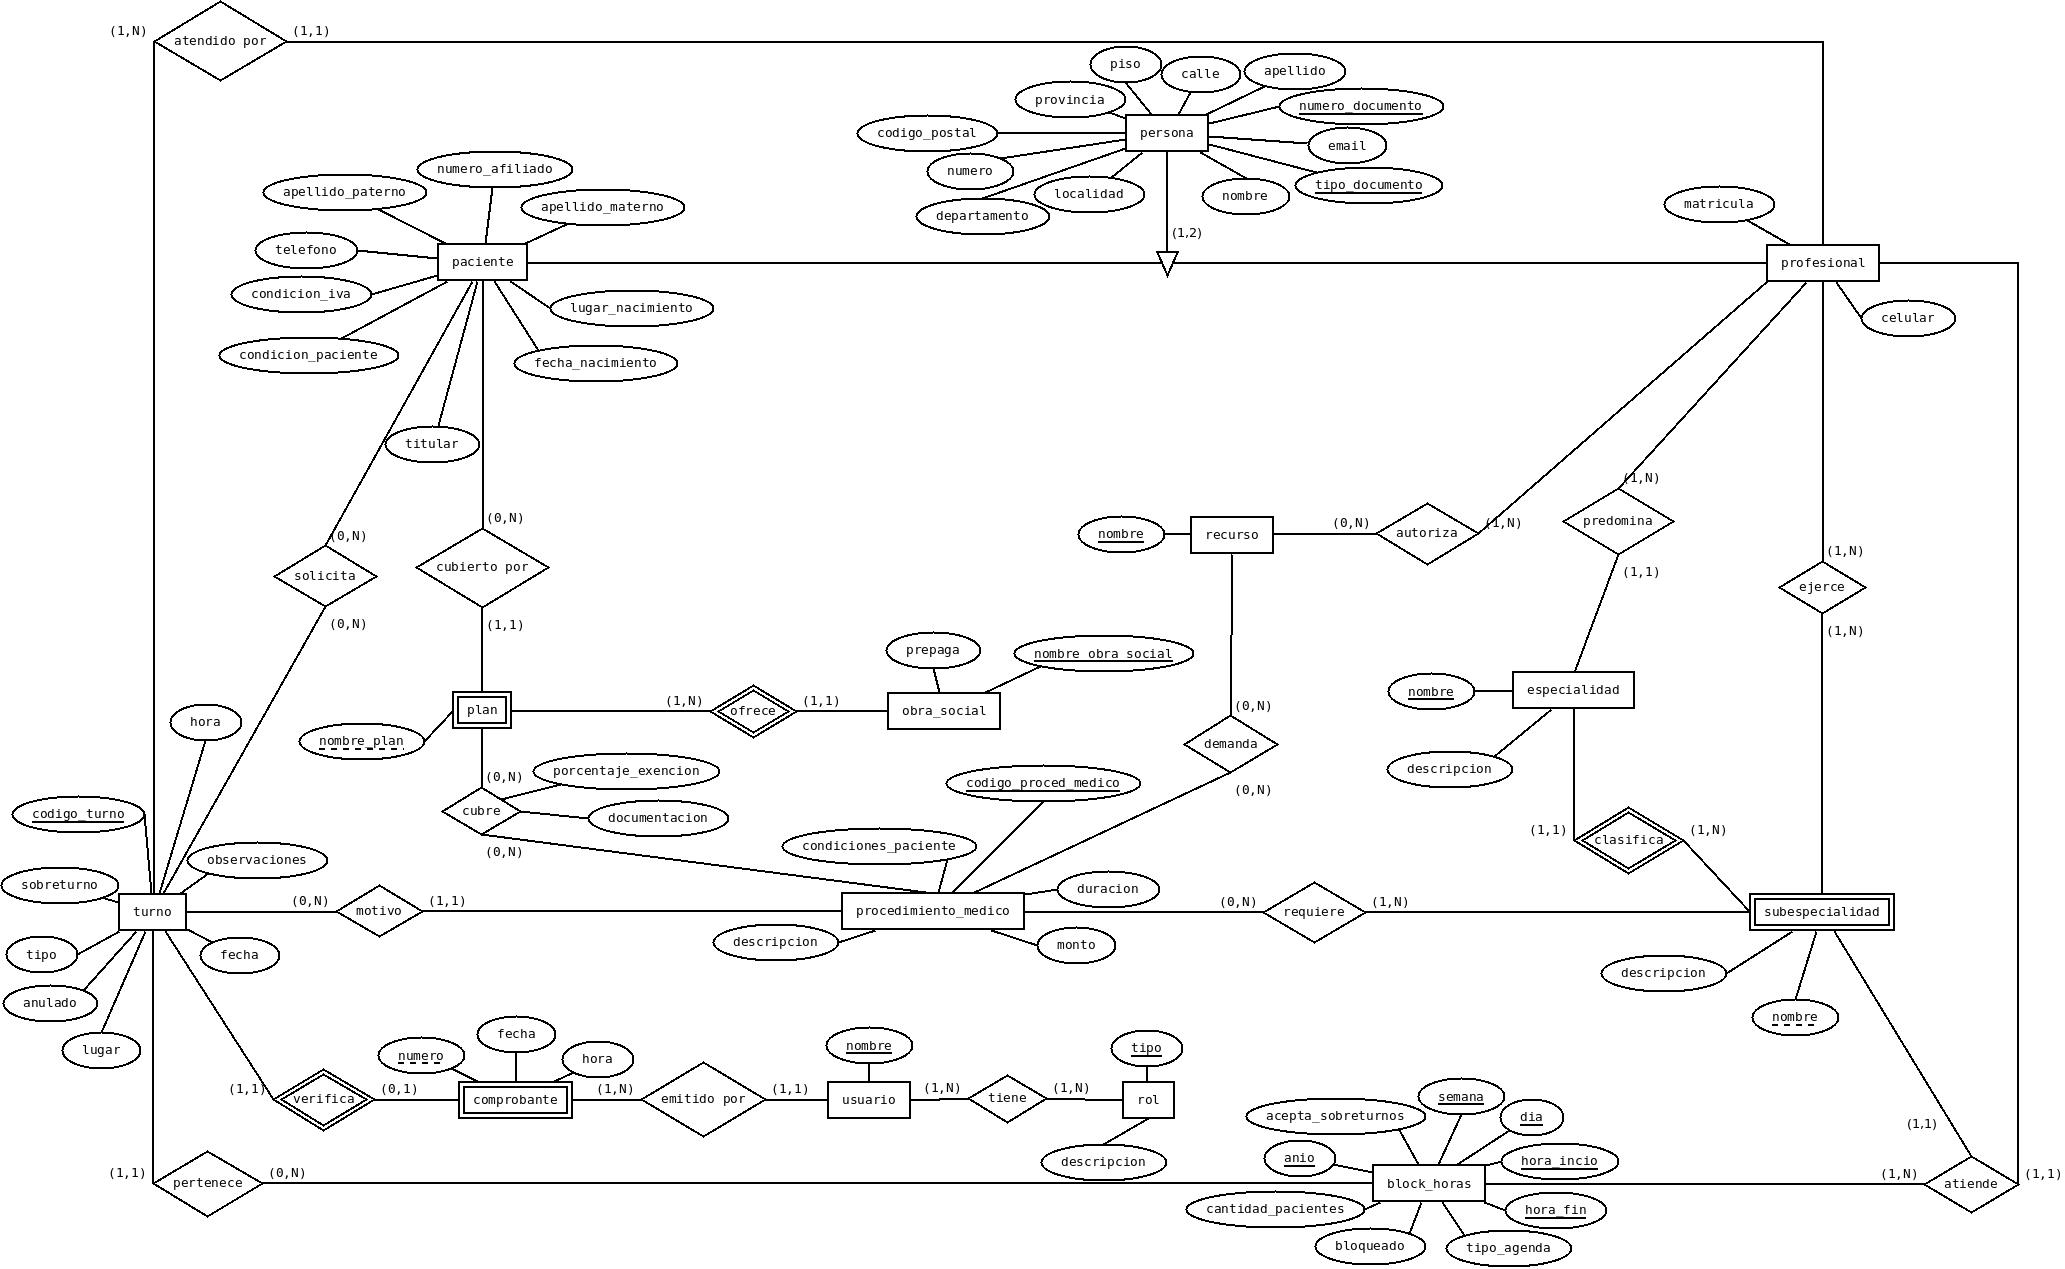
\includegraphics[width=1.4\textwidth, angle=90]{build/images/der.jpeg}
  \caption{Diagrama de entidad-interrelación} \label{fig:der}
\end{figure}

\FloatBarrier

\section{\textbf{Dependencias}}
\begin{enumerate}
\item Existe una dependencia de existencia de la entidad Turno con la entidad Block 
hora.

\item Existe una dependencia de identidad entre las entidades Plan y Obra social. 
Plan es una identidad débil, para poder identificarla utilizamos la razón social 
de la Obra Social (que es clave de la entidad fuerte) y como atributo discriminante 
el nombre del plan.

\item Existe una dependencia de identidad entre las entidades Especialidad y Subespecialidad. 
Subespecialidad es una identidad débil, para poder identificarla utilizamos el 
código de la Especialidad (que es clave de la entidad fuerte) y como atributo 
discriminante la descripción de la Subespecialidad.

\item Existe una dependencia de identidad entre las entidades Turno y Comprobante. 
Comprobante es una identidad débil, para poder identificarla utilizamos el código 
del Turno (que es clave de la entidad fuerte) y como atributo discriminante el 
número de Comprobante.\pagebreak{}
\end{enumerate}
\section{\textbf{Diccionario de datos}}

\subsection{\textbf{Entidades\label{HToc293405806}}}

\subsubsection{\textbf{Paciente}}

\textit{Definición}

Persona que recibe atención médica en el hospital. 

\textit{Especificación de atributos}

• Número de documento: número de documento del paciente.

• Tipo de documento: tipo de documento presentado por el paciente. Puede ser 
LE, LC, DNI, PASAPORTE.

• Número de afiliado: número asignado al paciente dentro del hospital.

• Nombre y apellido: nombre y apellido del paciente.

• Fecha de nacimiento: día, mes y año en que nació el afiliado.

• Lugar de nacimiento: ciudad o pueblo y país donde nació el paciente.

• Tipo beneficiario: indica la condición del paciente frente al hospital. Puede 
ser titular o adicional.

• Teléfono: número de teléfono del paciente.

• Email: dirección de correo electrónico del paciente.

• Condición IVA: condición del paciente frente al impuesto al valor agregado 
definido por la AFIP.

• Condición paciente: estado del paciente.

• Número de historia clínica: referencia el número de historia clínica que 
contiene tratamientos y diagnósticos del paciente.

\textit{Especificación de identificador único}

• Tipo documento

• DNI\label{HToc293405807}

\subsubsection{\textbf{Domicilio}}

\textit{Definición}

Lugar donde un PACIENTE o un PROFESIONAL tiene residencia.

\textit{Especificación de atributos}

• Código de domicilio: número entero que identifica al domicilio.

• Localidad: lugar perteneciente a una PROVINCIA.

• Provincia: subdivisión administrativa de un país.

• Calle: nombre de la calle correspondiente al domicilio.

• Número: número que identifica al terreno correspondiente al domicilio.

• Piso: nivel correspondiente al domicilio, en caso de que se trate de un edificio.

\textit{Especificación de identificador único}

• Código de domicilio\label{HToc293405808}

\subsubsection{\textbf{Profesional}}

\textit{Definición}

Un médico del hospital que diagnostica, atiende o trata a un PACIENTE.

\textit{Especificación de atributos}

• Nombre y apellido: nombre y apellido del profesional.

• Número de documento: número de documento del profesional.

• Tipo de documento: tipo de documento presentado por el profesional. Puede ser 
LE, LC, DNI, PASAPORTE.

• Celular: número de celular del profesional.

• Email: dirección de correo electrónico del profesional.

\textit{Especificación de identificador único}

• Tipo de documento

• Número de documento\label{HToc293405809}

\subsubsection{\textbf{Especialidad}}

\textit{Definición}

área de la medicina en que se especializa un PROFESIONAL.

\textit{Especificación de atributos}

• Código de especialidad: número entero que identifica la especialidad.

• Descripción: nombre de la especialidad.

\textit{Especificación de identificador único}

• Código de especialidad\label{HToc293405810}

\subsubsection{\textbf{Subespecialidad}}

\textit{Definición}

área dentro de la especialidad en que se especializa un PROFESIONAL. Depende de 
la especialidad.

\textit{Especificación de atributos}

• Descripción: nombre de la subespecialidad.

\textit{Especificación de identificador único}

• Código de especialidad

• Descripción\label{HToc293405811}

\subsubsection{\textbf{Acción médica}}

\textit{Definición}

Todo procedimiento médico, servicio, estudio o tratamiento brindado por el hospital. 
Incluye servicio de quirófano y camas.

\textit{Especificación de atributos}

• Código de acción médica: número entero que identifica la acción médica.

• Unidades: cantidad de unidades de tiempo asignadas a la acción médica. La 
unidad es 5 minutos.

• Descripción: denominación de la acción médica.

• Condiciones paciente: Texto de las condiciones médicas en la cual el paciente 
debe presentarse para realizarse el procedimiento médico a aplicar

\textit{Especificación de identificador único}

• Código de acción médica\label{HToc293405812}

\subsubsection{\textbf{Turno}}

\textit{Definición}

Fecha y hora en que se cita a un paciente que debe ser atendido en el hospital.

\textit{Especificación de atributos}

• Código de turno: número entero que identifica al turno.

• Fecha turno: día, mes y año en que se cita al paciente.

• Hora turno: hora y minutos en que el paciente fue citado.

• Sobreturno: atributo que puede valer si o no según el turno sea un sobreturno 
o no lo sea.

• Bloquado: atributo que puede valer si o no según el turno se encuentre bloqueado 
o no por el profesional asignado al turno.

• Lugar: dónde se atenderá al paciente citado.

\textit{Especificación de identificador único}

• Código de turno\label{HToc293405813}

\subsubsection{\textbf{Plan}}

\textit{Definición}

Prestaciones y servicios que ofrece una obra social determinada.

\textit{Especificación de atributos}

• Nombre: denominación del plan

\textit{Especificación de identificador único}

• Razón social de la obra social asociada

• Nombre del plan\label{HToc293405814}

\subsubsection{\textbf{Obra social}}

\textit{Definición}

Entidad que recibe aportes de un paciente y la brinda cobertura.

\textit{Especificación de atributos}

• Tipo de entidad: si la obra social es prepaga o pertenece a un sindicato.

• Razón social: denominacion legal de la obra social

\textit{Especificación de identificador único}

• Razón social\label{HToc293405815}

\subsubsection{\textbf{Block horas}}

\textit{Definición}

Designa los días y horarios en que un PROFESIONAL estará disponible para atender 
PACIENTES.

\textit{Especificación de atributos}

• Código de block de hora: número entero que identifica al block de horas.

• Hora desde: hora en que el PROFESIONAL comienza a atender PACIENTES.

• Hora desde: hora en que el PROFESIONAL finaliza la atención de PACIENTES.

• Día: día de la semana en que atiende el PROFESIONAL.

• Semana: semana del año en que es válido el block.

• Tipo de turno: indica características de los turnos que se generan a partir 
del block. Puede ser primera vez, visita subsiguiente, demanda espontánea.

• Tipo de agenda: indica la modalidad de atención de PACIENTES. Puede ser por 
orden de llegada o sin orden en particular.

• Bloqueado: permite indicar si un block está bloqueado por un PROFESIONAL o 
no.

• Acepta sobreturnos: vale sí si el PROFESIONAL decide aceptar sobreturnos dentro 
del block de horas, no si no.

• Acepta turnos fuera de agenda: toma el valor sí si el PROFESIONAL aceptará 
turnos fuera de agenda durante el horario del block, no, si no.

• Cantidad de pacientes: número de pacientes que el PROFESIONAL atenderá durante 
el tiempo que dure el block de horas.

\textit{Especificación de identificador único}

• Código de block de hora\label{HToc293405816}

\subsubsection{\textbf{Comprobante}}

\textit{Definición}

Contiene información relacionada con el turno que se conoce al momento que un 
PACIENTE reserva un turno.

\textit{Especificación de atributos}

• Número de comprobante: número entero que identifica el comprobante asociado 
al turno.

• Fecha de alta: fecha de alta del turno.

• Usuario: nombre del usuario que dio de alta el turno en el sistema.

\textit{Especificación de identificador único}

• Número de comprobante\label{HToc293405817}

\subsection{\textbf{Interrelaciones\label{HToc293405818}}}

\subsubsection{\textbf{Vive en}}

\textit{Definición}

Relaciona a un PROFESIONAL o un PACIENTE con el DOMICILIO donde reside.

\textit{Especificación de atributos}

-

\textit{Especificación de identificador único}

• Tipo de documento (PACIENTE)

• Número de documento (PACIENTE)

• Tipo de documento (PROFESIONAL)

• Número de documento (PROFESIONAL)\label{HToc293405819}

\subsubsection{\textbf{Se atiende}}

\textit{Definición}

Asocia a un PACIENTE y al TURNO que le ha sido asignado.

\textit{Especificación de atributos}

-

\textit{Especificación de identificador único}

• Tipo de documento

• Número de documento

• Código de turno\label{HToc293405820}

\subsubsection{\textbf{Asignado a}}

\textit{Definición}

Relaciona al PROFESIONAL con los TURNOS que le hayan sido asignados.

\textit{Especificación de atributos}

-

\textit{Especificación de identificador único}

• Código de turno\label{HToc293405821}

\subsubsection{\textbf{Se realiza}}

\textit{Definición}

Indica qué ACCIÓN MÉDICA se realizará en un TURNO.

\textit{Especificación de atributos}

-

\textit{Especificación de identificador único}

• Código de turno\label{HToc293405822}

\subsubsection{\textbf{Cubierto por}}

\textit{Definición}

Indica qué PLAN de OBRA SOCIAL cubre a un PACIENTE.

\textit{Especificación de atributos}

-

\textit{Especificación de identificador único}

• Tipo de documento

• Número de documento\label{HToc293405823}

\subsubsection{\textbf{Convenio}}

\textit{Definición}

Indica las caracterísiticas del convenio que tiene la el hospital con el PLAN 
de una OBRA SOCIAL determinada en relación a una ACCIÓN MÉDICA.

\textit{Especificación de atributos}

• Documentación requerida: Texto de la documentación del convenio, en la cual 
indica lo que el paciente debe presentar para realizarse el procedimiento médico 
a aplicar.

• Monto: cantidad de dinero aportado en el plan para la ACCIÓN MÉDICA. Es calculable.

• Porcentaje de exención: indica qué porcentaje del total del monto requerido 
para la ACCIÓN MÉDICA es cubierto por el PLAN.

\textit{Especificación de identificador único}

• Código de acción médica

• Razón social

• Nombre plan\label{HToc293405824}

\subsubsection{\textbf{Autorización}}

\textit{Definición}

Indica qué ACCIONes MÉDICAS un PROFESIONAL está autorizado a realizar.

\textit{Especificación de atributos}

-

\textit{Especificación de identificador único}

• Código de acción médica

• Tipo de documento

• Número de documento\label{HToc293405825}

\subsubsection{\textbf{Realizada por}}

\textit{Definición}

Indica qué SUBESPECIALIDAD realizará una ACCIÓN MEDICA.

\textit{Especificación de atributos}

-

\textit{Especificación de identificador único}

• Código de acción médica

• Código de especialidad

• Descripción de subespecialidad\label{HToc293405826}

\subsubsection{\textbf{Tiene}}

\textit{Definición}

Indica qué SUBESPECIALIDADes tiene un PROFESIONAL del hospital.

\textit{Especificación de atributos}

\textit{Especificación de identificador único}

• Código de especialidad

• Descripción de subespecialidad

• Tipo de documento

• Número de documento\label{HToc293405827}

\subsubsection{\textbf{Prevalece}}

\textit{Definición}

Permite modelar el requerimiento de que un PROFESIONAL solo puede tener una ESPECIALIDAD 
que prevalezca.

\textit{Especificación de atributos}

-

\textit{Especificación de identificador único}

• Tipo de documento

• Número de documento\label{HToc293405828}

\subsubsection{\textbf{Comprende}}

\textit{Definición}

Indica los TURNOs que componen un BLOCK HORA.

\textit{Especificación de atributos}

-

\textit{Especificación de identificador único}

• Código de turno\label{HToc293405829}

\subsubsection{\textbf{Define}}

\textit{Definición}

Indica a qué PROFESIONAL, desempeñando qué SUBESPECIALIDAD definió un BLOCK 
HORAS determinado.

\textit{Especificación de atributos}

-

\textit{Especificación de identificador único}

• Tipo de documento (PACIENTE)

• Número de documento (PACIENTE)

• Tipo de documento (PROFESIONAL)

• Número de documento (PROFESIONAL)

• Código de block horas\pagebreak{}\label{HToc293405830}

\section{\textbf{Modelo relacional\label{HToc293405831}}}

\subsection{\textbf{Diseño del modelo\label{HToc293405832}}}

\subsubsection{\textbf{Domicilio}}

DOMICILIO(\emph{codigo\_domicilio}, localidad, número, provincia, calle, piso);
\begin{itemize}
\item PK: (codigo\_domicilio)

\item FK: -

\item CC:

o (codigo\_domicilio)

\item ATRIBUTOS CON VALORES NULOS: -\label{HToc293405833}
\end{itemize}

\subsubsection{\textbf{Obra social}}

OBRA\_SOCIAL(\emph{razon\_social}, tipo\_entidad);

\begin{itemize}
\item PK: (razon social)

\item FK: -

\item CC:

o (razon\_social)

\item ATRIBUTOS CON VALORES NULOS: -\label{HToc293405834}
\end{itemize}

\subsubsection{\textbf{Plan}}

PLAN(\emph{razon\_social}, nombre\_plan);

\begin{itemize}
\item PK: (razon social, nombre\_plan)

\item FK: (razon\_social)

\item CC:

o (razon social, nombre\_plan)

\item ATRIBUTOS CON VALORES NULOS: -\label{HToc293405835}
\end{itemize}

\subsubsection{\textbf{Paciente}}

PACIENTE(\emph{tipo\_doc\_paciente, numero\_doc\_paciente}, numero\_afiliado, fecha\_nacimiento, 
lugar\_nacimiento, tipo\_beneficiario, telefono, email, condicion\_iva, condicion\_paciente, 
numero\_historia\_clinica, apellido\_nombre, codigo\_domicilio, razon\_social, 
 nombre\_plan);

\begin{itemize}
\item PK: (tipo\_doc\_paciente, numero\_doc\_paciente)

\item FK: 

o (codigo\_domicilio) 

o (razon\_social , nombre\_plan)

\item CC:

o (tipo\_doc\_paciente, numero\_doc\_paciente)

o (razon\_social, numero\_afiliado)

\item ATRIBUTOS CON VALORES NULOS:  fecha\_nacimiento, lugar\_nacimiento, tipo\_beneficiario, 
email, condicion\_iva, condicion\_paciente\label{HToc293405836}
\end{itemize}

\subsubsection{\textbf{Acción médica}}

ACCION\_MEDICA(\emph{codigo\_accion\_medica}, unidades, condiciones\_paciente, 
descripción);

\begin{itemize}
\item PK: (codigo\_accion\_medica)

\item FK:-

\item CC:

o (codigo\_accion\_medica)

\item ATRIBUTOS CON VALORES NULOS:  condiciones\_paciente.\label{HToc293405837}
\end{itemize}

\subsubsection{\textbf{Especialidad}}

ESPECIALIDAD(\emph{codigo\_especialidad}, descripción);

\begin{itemize}
\item PK: (codigo\_especialidad)

\item FK:-

\item CC:

o (codigo\_especialidad)

\item ATRIBUTOS CON VALORES NULOS: - \label{HToc293405838}
\end{itemize}

\subsubsection{\textbf{Subespecialidad}}

SUBESPECIALIDAD(\emph{codigo\_especialidad}, descripcion\_subespecialidad);

\begin{itemize}
\item PK: (codigo\_especialidad, descripcion\_subespecialidad)

\item FK: (codigo\_especialidad)

\item CC:

o (codigo\_especialidad, descripcion\_subespecialidad)

\item ATRIBUTOS CON VALORES NULOS: -\label{HToc293405839}
\end{itemize}

\subsubsection{\textbf{Profesional}}

PROFESIONAL(\emph{tipo\_doc\_profesional, numero\_doc\_profesional}, apellido\_nombre, 
email, número\_matrícula, celular,\textit{\textbf{ }}codigo\_domicilio, codigo\_especialidad)

\begin{itemize}
\item PK: (tipo\_doc\_profesional, numero\_doc\_profesional)

\item FK: 

o (codigo\_domicilio)

o (código\_especialidad)

\item CC:

o (tipo\_doc\_profesional, numero\_doc\_profesional) 

\item ATRIBUTOS CON VALORES NULOS:  email.\label{HToc293405840}
\end{itemize}

\subsubsection{\textbf{Block horas}}

BLOCK\_HORAS(\emph{codigo\_block\_horas}, día, semana, hora\_desde,hora\_hasta, 
acepta\_sobreturnos, acepta\_fuera\_agenda, bloqueado, tipo\_turno, tipo\_agenda, 
cantidad\_pacientes, unidades,\emph{ }tipo\_doc\_profesional, numero\_doc\_profesional, 
codigo\_especialidad, descripcion\_subespecialidad);

\begin{itemize}
\item PK: (codigo\_block\_horas)

\item FK: 

o (tipo\_doc\_profesional, numero\_doc\_profesional, codigo\_especialidad, descripcion\_subespecialidad)

\item CC:

o (codigo\_block\_horas)

\item ATRIBUTOS CON VALORES NULOS: acepta\_sobreturnos, acepta\_fuera\_agenda, bloqueado, 
tipo\_turno, tipo\_agenda, cantidad\_pacientes, unidades.\label{HToc293405841}
\end{itemize}

\subsubsection{\textbf{Turno}}

TURNO(\emph{código\_turno}, fecha\_turno, hora\_turno, observaciones, lugar, sobreturno, 
bloqueado, código\_block\_horas,código\_acción\_medica);

\begin{itemize}
\item PK: (codigo\_turno)

\item FK: 

o (codigo\_block\_horas)

o (codigo\_accion\_medica)

\item CC:

o (codigo\_turno)

\item ATRIBUTOS CON VALORES NULOS:  observaciones, lugar.\label{HToc293405842}
\end{itemize}

\subsubsection{\textbf{Comprobante}}

COMPROBANTE(\emph{código\_turno}, número\_comprobante, fecha\_alta, usuario);

\begin{itemize}
\item PK: (codigo\_turno, numero\_comprobante)

\item FK: 

o (codigo\_turno)

\item CC:

o (codigo\_turno, numero\_comprobante)

\item ATRIBUTOS CON VALORES NULOS:  fecha alta, usuario.
\end{itemize}

\textbf{Vive en (profesional)}

\textit{Diseño 1}

VIVE\_EN\_PROFESIONAL(\emph{ tipo\_doc\_profesional, numero\_doc\_profesional, 
}codigo\_domicilio)

\begin{itemize}
\item PK: (tipo\_doc\_profesional, numero\_doc\_profesional)

\item FK: 

o (codigo\_domicilio)

o (tipo\_doc\_profesional, numero\_doc\_profesional)

\item CC:

o (tipo\_doc\_profesional, numero\_doc\_profesional)

\item ATRIBUTOS CON VALORES NULOS: -
\end{itemize}

DOMICILIO(\emph{codigo\_domicilio}, localidad, número, provincia, calle, piso)

PROFESIONAL(\emph{tipo\_doc\_profesional, numero\_doc\_profesional}, apellido\_nombre, 
email, número\_matrícula, celular, codigo\_especialidad)

\textit{Diseño 2}

DOMICILIO(\emph{codigo\_domicilio}, localidad, número, provincia, calle, piso)

PROFESIONAL(\emph{tipo\_doc\_profesional, numero\_doc\_profesional}, apellido\_nombre, 
email, número\_matrícula, celular,\textit{\textbf{ }}codigo\_domicilio, codigo\_especialidad)

Se optó por el diseño 2 porque reduce el número de tablas.\label{HToc293405843}

\subsubsection{\textbf{Vive en (paciente)}}

\textit{Diseño 1}

VIVE\_EN\_PACIENTE(\emph{tipo\_doc\_paciente, numero\_doc\_paciente,} codigo\_domicilio)

\begin{itemize}
\item PK: (tipo\_doc\_paciente, numero\_doc\_paciente)

\item FK: 

o (codigo\_domicilio)

o (tipo\_doc\_paciente, numero\_doc\_paciente)

\item CC:

o (tipo\_doc\_paciente, numero\_doc\_paciente)

\item ATRIBUTOS CON VALORES NULOS: -
\end{itemize}

DOMICILIO(\emph{codigo\_domicilio}, localidad, número, provincia, calle, piso);

PACIENTE(\emph{tipo\_doc\_paciente, numero\_doc\_paciente}, numero\_afiliado, fecha\_nacimiento, 
lugar\_nacimiento, tipo\_beneficiario, telefono, email, condicion\_iva, condicion\_paciente, 
numero\_historia\_clinica, apellido\_nombre, razon\_social,  nombre\_plan);

\textit{Diseño 2}

DOMICILIO(\emph{codigo\_domicilio}, localidad, número, provincia, calle, piso);

PACIENTE(\emph{tipo\_doc\_paciente, numero\_doc\_paciente}, numero\_afiliado, fecha\_nacimiento, 
lugar\_nacimiento, tipo\_beneficiario, telefono, email, condicion\_iva, condicion\_paciente, 
numero\_historia\_clinica, apellido\_nombre, codigo\_domicilio, razon\_social, 
 nombre\_plan);

Se optó por el diseño 2 porque reduce el número de tablas.\label{HToc293405844}

\subsubsection{\textbf{Tiene\_Especialidad}}

TIENE\_ESPECIALIDAD(\emph{tipo\_doc\_profesional, numero\_doc\_profesional, codigo\_especialidad,} 
\emph{descripcion\_subespecialidad});

\begin{itemize}
\item PK: (tipo\_doc\_profesional, numero\_doc\_profesional, codigo\_especialidad, 
descripcion\_subespecialidad)

\item FK: 

o (tipo\_doc\_profesional, numero\_doc\_profesional)

o (codigo\_especialidad, descripcion\_subespecialidad)

\item CC:

o (tipo\_doc\_profesional, numero\_doc\_profesional, codigo\_especialidad, descripcion\_subespecialidad)

\item ATRIBUTOS CON VALORES NULOS:  -.
\end{itemize}

PROFESIONAL(\emph{tipo\_doc\_profesional, numero\_doc\_profesional}, apellido\_nombre, 
email, número\_matrícula, celular,\textit{\textbf{ }}codigo\_domicilio, codigo\_especialidad)

SUBESPECIALIDAD(\emph{codigo\_especialidad, }descripcion\_subespecialidad);\label{HToc293405845}

\subsubsection{\textbf{Prevalece}}

\textit{Diseño 1}

PREVALECE(\emph{tipo\_doc\_profesional, numero\_doc\_profesional}\textit{, }codigo\_especialidad);

\begin{itemize}
\item PK: (tipo\_doc\_profesional, numero\_doc\_profesional)

\item FK: 

o (tipo\_doc\_profesional, numero\_doc\_profesional)

o (codigo\_especialidad)

\item CC:

o (tipo\_doc\_profesional, numero\_doc\_profesional)

\item ATRIBUTOS CON VALORES NULOS:  -.
\end{itemize}

PROFESIONAL(\emph{tipo\_doc\_profesional, numero\_doc\_profesional}, apellido\_nombre, 
email, número\_matrícula, celular\textit{\textbf{, }}codigo\_domicilio);

ESPECIALIDAD(\emph{codigo\_especialidad}, descripción);

\textit{Diseño 2}

PROFESIONAL(\emph{tipo\_doc\_profesional, numero\_doc\_profesional}, apellido\_nombre, 
email, número\_matrícula, celular\textit{\textbf{, }}codigo\_domicilio,\textit{\textbf{ 
}}codigo\_especialidad);

ESPECIALIDAD(\emph{codigo\_especialidad}, descripción);

Se optó por el diseño 2 porque reduce el número de tablas.\label{HToc293405846}

\subsubsection{\textbf{Convenio}}

CONVENIO(\emph{codigo\_accion\_medica, razon\_social , nombre\_plan}, porcentaje\_exencion, 
documentación\_requerida, monto);

\begin{itemize}
\item PK: (codigo\_accion\_medica, razon social, nombre\_plan)

\item FK: 

o (codigo\_accion\_medica)

o (razon\_social,  nombre\_plan)

\item CC:

o (codigo\_accion\_medica, razon social, nombre\_plan)

\item ATRIBUTOS CON VALORES NULOS:  -

ACCION\_MEDICA(\emph{codigo\_accion\_medica}, unidades, condiciones\_paciente, 
descripción);
\end{itemize}

PLAN(\emph{razon\_social, }nombre\_plan);\label{HToc293405847}

\subsubsection{\textbf{Autorización}}

AUTORIZACIÓN(\emph{código\_accion\_medica, tipo\_doc\_profesional, numero\_doc\_profesional});

\begin{itemize}
\item PK: (codigo\_accion\_medica, tipo\_doc\_profesional, numero\_doc\_profesional)

\item FK: 

o (codigo\_accion\_medica)

o (tipo\_doc\_profesional, numero\_doc\_profesional)

\item CC:

o (codigo\_accion\_medica, tipo\_doc\_profesional, numero\_doc\_profesional)

\item ATRIBUTOS CON VALORES NULOS:  -.
\end{itemize}

ACCION\_MEDICA(\emph{codigo\_accion\_medica}, unidades, condiciones\_paciente, 
descripción);

PROFESIONAL(\emph{tipo\_doc\_profesional, numero\_doc\_profesional}, apellido\_nombre, 
email, número\_matrícula, celular\textit{\textbf{, }}codigo\_domicilio, codigo\_especialidad);\label{HToc293405848}

\subsubsection{\textbf{Realiza\_Accion}}

REALIZA\_ACCION(\emph{codigo\_accion\_medica, codigo\_especialidad, descripcion\_subespecialidad});

\begin{itemize}
\item PK: (codigo\_accion\_medica, codigo\_especialidad, descripcion\_subespecialidad)

\item FK: 

o (codigo\_accion\_medica)

o (codigo\_especialidad, descripcion\_subespecialidad)

\item CC:

o (codigo\_accion\_medica, codigo\_especialidad, descripcion\_subespecialidad)

\item ATRIBUTOS CON VALORES NULOS:  -.
\end{itemize}

ACCION\_MEDICA(\emph{codigo\_accion\_medica}, unidades, condiciones\_paciente, 
descripción);

SUBESPECIALIDAD(\emph{codigo\_especialidad, }descripcion\_subespecialidad);\label{HToc293405849}

\subsubsection{\textbf{Comprende}}

\textit{Diseño 1}

COMPRENDE(\emph{codigo\_turno} , código\_block\_horas);

\begin{itemize}
\item PK: (codigo\_turno)

\item FK: 

o (codigo turno)

o (codigo\_block\_horas)

\item CC:

o (codigo\_turno)

\item ATRIBUTOS CON VALORES NULOS:  -.
\end{itemize}

TURNO(\emph{código\_turno},fecha\_turno,hora\_turno,observaciones,lugar,sobreturno,bloqueado, 
código\_acción\_medica);

BLOCK\_HORAS(\emph{codigo\_block\_horas}, día, semana, hora\_desde, hora\_hasta, 
acepta\_sobreturnos, acepta\_fuera\_agenda, bloqueado, tipo\_turno, tipo\_agenda, 
cantidad\_pacientes, unidades,\emph{ }tipo\_doc\_profesional, numero\_doc\_profesional, 
codigo\_especialidad, descripcion\_subespecialidad);

\textit{Diseño 2}

TURNO(\emph{código\_turno}, fecha\_turno, hora\_turno,observaciones, lugar, sobreturno, 
bloqueado, código\_block\_horas, código\_acción\_medica);

BLOCK\_HORAS(\emph{codigo\_block\_horas}, día, semana, hora\_desde,hora\_hasta, 
acepta\_sobreturnos, acepta\_fuera\_agenda, bloqueado, tipo\_turno, tipo\_agenda, 
cantidad\_pacientes, unidades,\emph{ }tipo\_doc\_profesional, numero\_doc\_profesional, 
codigo\_especialidad, descripcion\_subespecialidad);

Se optó por el diseño 2 porque reduce el número de tablas.\label{HToc293405850}

\subsubsection{\textbf{Se realiza}}

\textit{Diseño 1}

SE\_REALIZA(\emph{código\_turno, }código\_accion\_medica);

\begin{itemize}
\item PK: (codigo\_turno)

\item FK: 

o (codigo\_accion\_medica)

o (codigo turno)

\item CC:

o (codigo\_turno)

\item ATRIBUTOS CON VALORES NULOS:-
\end{itemize}

TURNO(\emph{código\_turno}, fecha\_turno, hora\_turno, observaciones, lugar, sobreturno, 
bloqueado, código\_block\_horas);

ACCION\_MEDICA(\emph{código\_accion\_medica}, unidades, condiciones\_paciente, 
descripción);

\textit{Diseño 2}

TURNO(\emph{código\_turno}, fecha\_turno, hora\_turno, observaciones, lugar, sobreturno 
,bloqueado, código\_block\_horas, codigo\_accion\_medica);

ACCION\_MEDICA(\emph{código\_accion\_medica}, unidades, condiciones\_paciente, 
descripción);

Se opto por el diseño 2 porque reduce el número de tablas.\label{HToc293405851}

\subsubsection{\textbf{Define\label{HToc293405852}}}

\subsubsection{\textit{Diseño 1}}

DEFINE\_BLOCK\_HORAS (\emph{codigo\_block\_horas},  tipo\_doc\_profesional, numero\_doc\_profesional, 
codigo\_especialidad, descripcion\_subespecialidad);

\begin{itemize}
\item PK: (codigo\_block\_horas)

\item FK: 

o (tipo\_doc\_profesional, numero\_doc\_profesional, codigo\_especialidad, descripcion\_subespecialidad)

o (codigo\_block\_horas)

\item CC:

o (codigo\_block\_horas)

\item ATRIBUTOS CON VALORES NULOS:-
\end{itemize}

BLOCK\_HORAS(\emph{codigo\_block\_horas}, día, semana, hora\_desde,hora\_hasta, 
acepta\_sobreturnos, acepta\_fuera\_agenda, bloqueado, tipo\_turno, tipo\_agenda, 
cantidad\_pacientes, unidades);

TIENE\_ESPECIALIDAD(\emph{tipo\_doc\_profesional, numero\_doc\_profesional, codigo\_especialidad,} 
\emph{descripcion\_subespecialidad})

\textit{Diseño 2}

BLOCK\_HORAS(\emph{codigo\_block\_horas}, día, semana, hora\_desde,hora\_hasta, 
acepta\_sobreturnos, acepta\_fuera\_agenda, bloqueado, tipo\_turno, tipo\_agenda, 
cantidad\_pacientes, unidades,\emph{ }tipo\_doc\_profesional, numero\_doc\_profesional, 
codigo\_especialidad, descripcion\_subespecialidad);

TIENE\_ESPECIALIDAD(\emph{tipo\_doc\_profesional, numero\_doc\_profesional, codigo\_especialidad,} 
\emph{descripcion\_subespecialidad})

Se optó por el diseño 2 porque reduce el número de tablas.\label{HToc293405853}

\subsubsection{\textbf{Se atiende}}

SE\_ATIENDE(\emph{tipo\_doc\_paciente, numero\_doc\_paciente, código\_turno})

\begin{itemize}
\item PK: (tipo\_doc\_paciente, numero\_doc\_paciente, codigo\_turno)

\item FK: 

o (codigo\_turno)

o (tipo\_doc\_paciente, numero\_doc\_paciente)

\item CC:

o (tipo\_doc\_paciente, numero\_doc\_paciente, código\_turno)

\item ATRIBUTOS CON VALORES NULOS:  -.
\end{itemize}

TURNO(\emph{código\_turno}, fecha\_turno, hora\_turno, observaciones, lugar, sobreturno, 
bloqueado, código\_block\_horas,código\_acción\_medica);

PACIENTE(\emph{tipo\_doc\_paciente, numero\_doc\_paciente}, numero\_afiliado, fecha\_nacimiento, 
lugar\_nacimiento, tipo\_beneficiario, telefono, email, condicion\_iva, condicion\_paciente, 
numero\_historia\_clinica, apellido\_nombre, codigo\_domicilio, razon\_social, 
 nombre\_plan);\label{HToc293405854}

\subsubsection{\textbf{Turno\_Asignado}}

\textit{Diseño 1}

TURNO\_ASIGNADO(\emph{código\_turno}, tipo\_doc\_profesional, numero\_doc\_profesional);

\begin{itemize}
\item PK: (codigo\_turno)

\item FK: 

o (codigo\_turno)

o (tipo\_doc\_profesional, numero\_doc\_profesional)

\item CC:

o (codigo\_turno)

\item ATRIBUTOS CON VALORES NULOS: -
\end{itemize}

TURNO(\emph{código\_turno}, fecha\_turno, hora\_turno, observaciones, lugar, sobreturno, 
bloqueado, código\_block\_horas,código\_acción\_medica);

PROFESIONAL(\emph{tipo\_doc\_profesional, numero\_doc\_profesional}, apellido\_nombre, 
email, número\_matrícula, celular,\textit{\textbf{ }}codigo\_domicilio, codigo\_especialidad)

\textit{Diseño 2}

TURNO(\emph{código\_turno}, fecha\_turno, hora\_turno, observaciones, lugar, sobreturno, 
bloqueado, código\_block\_horas,código\_acción\_medica, tipo\_doc\_profesional, 
numero\_doc\_profesional)

PROFESIONAL(\emph{tipo\_doc\_profesional, numero\_doc\_profesional}, apellido\_nombre, 
email, número\_matrícula, celular,\textit{\textbf{ }}codigo\_domicilio, codigo\_especialidad)

Se optó por el diseño 1 porque facilita las búsquedas de turnos asignados a 
un profesional.\pagebreak{}\label{HToc293405855}

\subsection{\textbf{Diagrama de tablas}}\pagebreak{}\label{HToc293405856}

\subsection{\textbf{DDL}}

create table domicilio(

codigo\_domicilio INTEGER NOT NULL, 

provincia  CHAR(10),

localidad  CHAR(10),

calle   CHAR(10),

numero  CHAR(10),

piso   CHAR(10),

PRIMARY KEY (codigo\_domicilio)

);

create table obra\_social(

razon\_social  CHAR(30) NOT NULL, 

tipo\_entidad  CHAR(30),

PRIMARY KEY (razon\_social)

); 

create table plan(

razon\_social  CHAR(30) NOT NULL,

nombre\_plan  CHAR(10) NOT NULL, 

PRIMARY KEY (razon\_social, nombre\_plan),

FOREIGN KEY (razon\_social) REFERENCES obra\_social

);  

create table especialidad(

codigo\_especialidad INTEGER NOT NULL, 

descripcion  CHAR(50),

PRIMARY KEY (codigo\_especialidad)

);  

create table subespecialidad(

codigo\_especialidad  INTEGER NOT NULL, 

descripcion\_subespecialidad CHAR(50) NOT NULL,

PRIMARY KEY (codigo\_especialidad, descripcion\_subespecialidad),

FOREIGN KEY (codigo\_especialidad) REFERENCES especialidad

);

create table accion\_medica(

codigo\_accion\_medica  CHAR(10) NOT NULL, 

unidades   INTEGER

condiciones\_paciente  CHAR(50),

descripcion   CHAR(100),

PRIMARY KEY (codigo\_accion\_medica)

); 

create table convenio(

nombre\_plan   CHAR(10) NOT NULL, 

razon\_social   CHAR(30) NOT NULL,

codigo\_accion\_medica  CHAR(10) NOT NULL,

documentacion\_requerida CHAR(100),

monto    DECIMAL(10,2),

porcentaje\_exencion  DECIMAL(10,2),

PRIMARY KEY (nombre\_plan , razon\_social, codigo\_accion\_medica),

FOREIGN KEY (razon\_social , nombre\_plan) REFERENCES plan,

FOREIGN KEY (codigo\_accion\_medica) REFERENCES accion\_medica

); 

create table profesional(

tipo\_doc\_profesional  CHAR(10) NOT NULL,

numero\_doc\_profesional   INTEGER NOT NULL, 

apellido\_nombre  CHAR(50),

email    CHAR(20),

numero\_matricula  INTEGER,

celular    CHAR(10),

codigo\_especialidad  INTEGER,    

codigo\_domicilio   INTEGER,

PRIMARY KEY (tipo\_doc\_profesional, numero\_doc\_profesional),

FOREIGN KEY (codigo\_especialidad) REFERENCES especialidad,

FOREIGN KEY (codigo\_domicilio) REFERENCES domicilio

);

create table paciente(

tipo\_doc\_paciente     CHAR(10) NOT NULL, 

numero\_doc\_paciente  INTEGER NOT NULL,

numero\_afiliado  INTEGER NOT NULL,

fecha\_nacimiento  CHAR(10),

lugar\_nacimiento  CHAR(30),

tipo\_beneficiario  CHAR(10),    

telefono    CHAR(10) NOT NULL,    

email     CHAR(20),    

condicion\_iva    CHAR(10),

condicion\_paciente   CHAR(10),

numero\_historia\_clinica INTEGER NOT NULL,    

apellido\_nombre   CHAR(50) NOT NULL,    

nombre\_plan    CHAR(10),    

razon\_social    CHAR(30),

codigo\_domicilio  INTEGER,

PRIMARY KEY (tipo\_documento ,  numero\_doc\_paciente),

FOREIGN KEY (razon\_social , nombre\_plan) REFERENCES plan,

FOREIGN KEY (codigo\_domicilio) REFERENCES domicilio

); 

create table tiene\_especialidad(

tipo\_doc\_profesional  CHAR(10) NOT NULL,

numero\_doc\_profesional   INTEGER NOT NULL,

codigo\_especialidad  INTEGER NOT NULL, 

descripcion\_subespecialidad CHAR(50) NOT NULL,

PRIMARY KEY (tipo\_doc\_profesional, numero\_doc\_profesional, codigo\_especialidad, 
descripcion\_subespecialidad),

FOREIGN KEY (tipo\_doc\_profesional, numero\_doc\_profesional)     REFERENCES profesional,

FOREIGN KEY (codigo\_especialidad, descripcion\_subespecialidad) REFERENCES subespecialidad

);

create table autorizacion(

tipo\_doc\_profesional  CHAR(10) NOT NULL,

numero\_doc\_profesional   INTEGER NOT NULL,

codigo\_accion\_medica  CHAR(10) NOT NULL, 

PRIMARY KEY (tipo\_doc\_profesional, numero\_doc\_profesional, codigo\_accion\_medica),

FOREIGN KEY (tipo\_doc\_profesional, numero\_doc\_profesional)     REFERENCES profesional,

FOREIGN KEY (codigo\_accion\_medica) REFERENCES accion\_medica

); 

create table realiza\_accion(

codigo\_especialidad  INTEGER NOT NULL, 

descripcion\_subespecialidad CHAR(50) NOT NULL,

codigo\_accion\_medica  CHAR(10) NOT NULL, 

PRIMARY KEY (codigo\_especialidad, descripcion\_subespecialidad, codigo\_accion\_medica),

FOREIGN KEY (codigo\_especialidad, descripcion\_subespecialidad)     REFERENCES 
subespecialidad,

FOREIGN KEY (codigo\_accion\_medica) REFERENCES accion\_medica

);  

create table block\_horas(

codigo\_block\_horas     INTEGER NOT NULL, 

dia    CHAR(10) NOT NULL,

semana    CHAR(10) NOT NULL,

hora\_desde   CHAR(10) NOT NULL,

hora\_hasta   CHAR(10) NOT NULL,

acepta\_sobreturno  CHAR(1),    

acepta\_fuera\_agenda  CHAR(10),    

bloqueado    CHAR(1),    

unidades    CHAR(10),

tipo\_turno   CHAR(10),    

cantidad\_pacientes   INTEGER,

tipo\_doc\_profesional  CHAR(10) NOT NULL,

numero\_doc\_profesional   INTEGER NOT NULL,

codigo\_especialidad  INTEGER NOT NULL, 

descripcion\_subespecialidad CHAR(50) NOT NULL,    

PRIMARY KEY (codigo\_block\_horas),

FOREIGN KEY (tipo\_doc\_profesional, numero\_doc\_profesional,  codigo\_especialidad, 
descripcion\_subespecialidad) REFERENCES tiene\_especialidad

); 

create table turno(

codigo\_turno      INTEGER NOT NULL, 

fecha\_turno   DATETIME NOT NULL,

hora\_turno   DATETIME NOT NULL,

observaciones   CHAR(100),

lugar    CHAR(100),

sobreturno   CHAR(1),    

bloqueado    CHAR(1),    

codigo\_block\_horas  INTEGER,

codigo\_accion\_medica  CHAR(10),    

PRIMARY KEY (codigo\_turno),

FOREIGN KEY (codigo\_block\_horas) REFERENCES block\_horas,

FOREIGN KEY (codigo\_accion\_medica) REFERENCES accion\_medica

); 

create table se\_atiende(

tipo\_doc\_paciente  CHAR(10) NOT NULL,

numero\_doc\_paciente  INTEGER NOT NULL,

codigo\_turno   INTEGER NOT NULL,

PRIMARY KEY (tipo\_doc\_paciente, numero\_doc\_paciente, codigo\_turno),

FOREIGN KEY (tipo\_doc\_paciente, numero\_doc\_paciente) REFERENCES paciente,

FOREIGN KEY (codigo\_turno) REFERENCES turno

);

create table turno\_asignado(

tipo\_doc\_profesional  CHAR(10) NOT NULL,

numero\_doc\_profesional   INTEGER NOT NULL,

codigo\_turno   INTEGER NOT NULL,

PRIMARY KEY (tipo\_doc\_profesional, numero\_doc\_profesional, codigo\_turno),

FOREIGN KEY (tipo\_doc\_profesional, numero\_doc\_profesional) REFERENCES profesional,

FOREIGN KEY (codigo\_turno) REFERENCES turno

);

create table comprobante(

codigo\_turno   INTEGER NOT NULL,

numero\_comprobante  INTEGER NOT NULL, 

fecha\_alta   DATETIME NOT NULL,

usuario    CHAR(20),

PRIMARY KEY (codigo\_turno, numero\_comprobante),

FOREIGN KEY (codigo\_turno) REFERENCES turno

);

\newpage

\subsection{Scripts de creación}

%%Acá se deberían incluir los scripts de creación.

\clearpage

\part{Apéndice}
\appendix

\section{Enunciado original}\label{sec:enunciado}
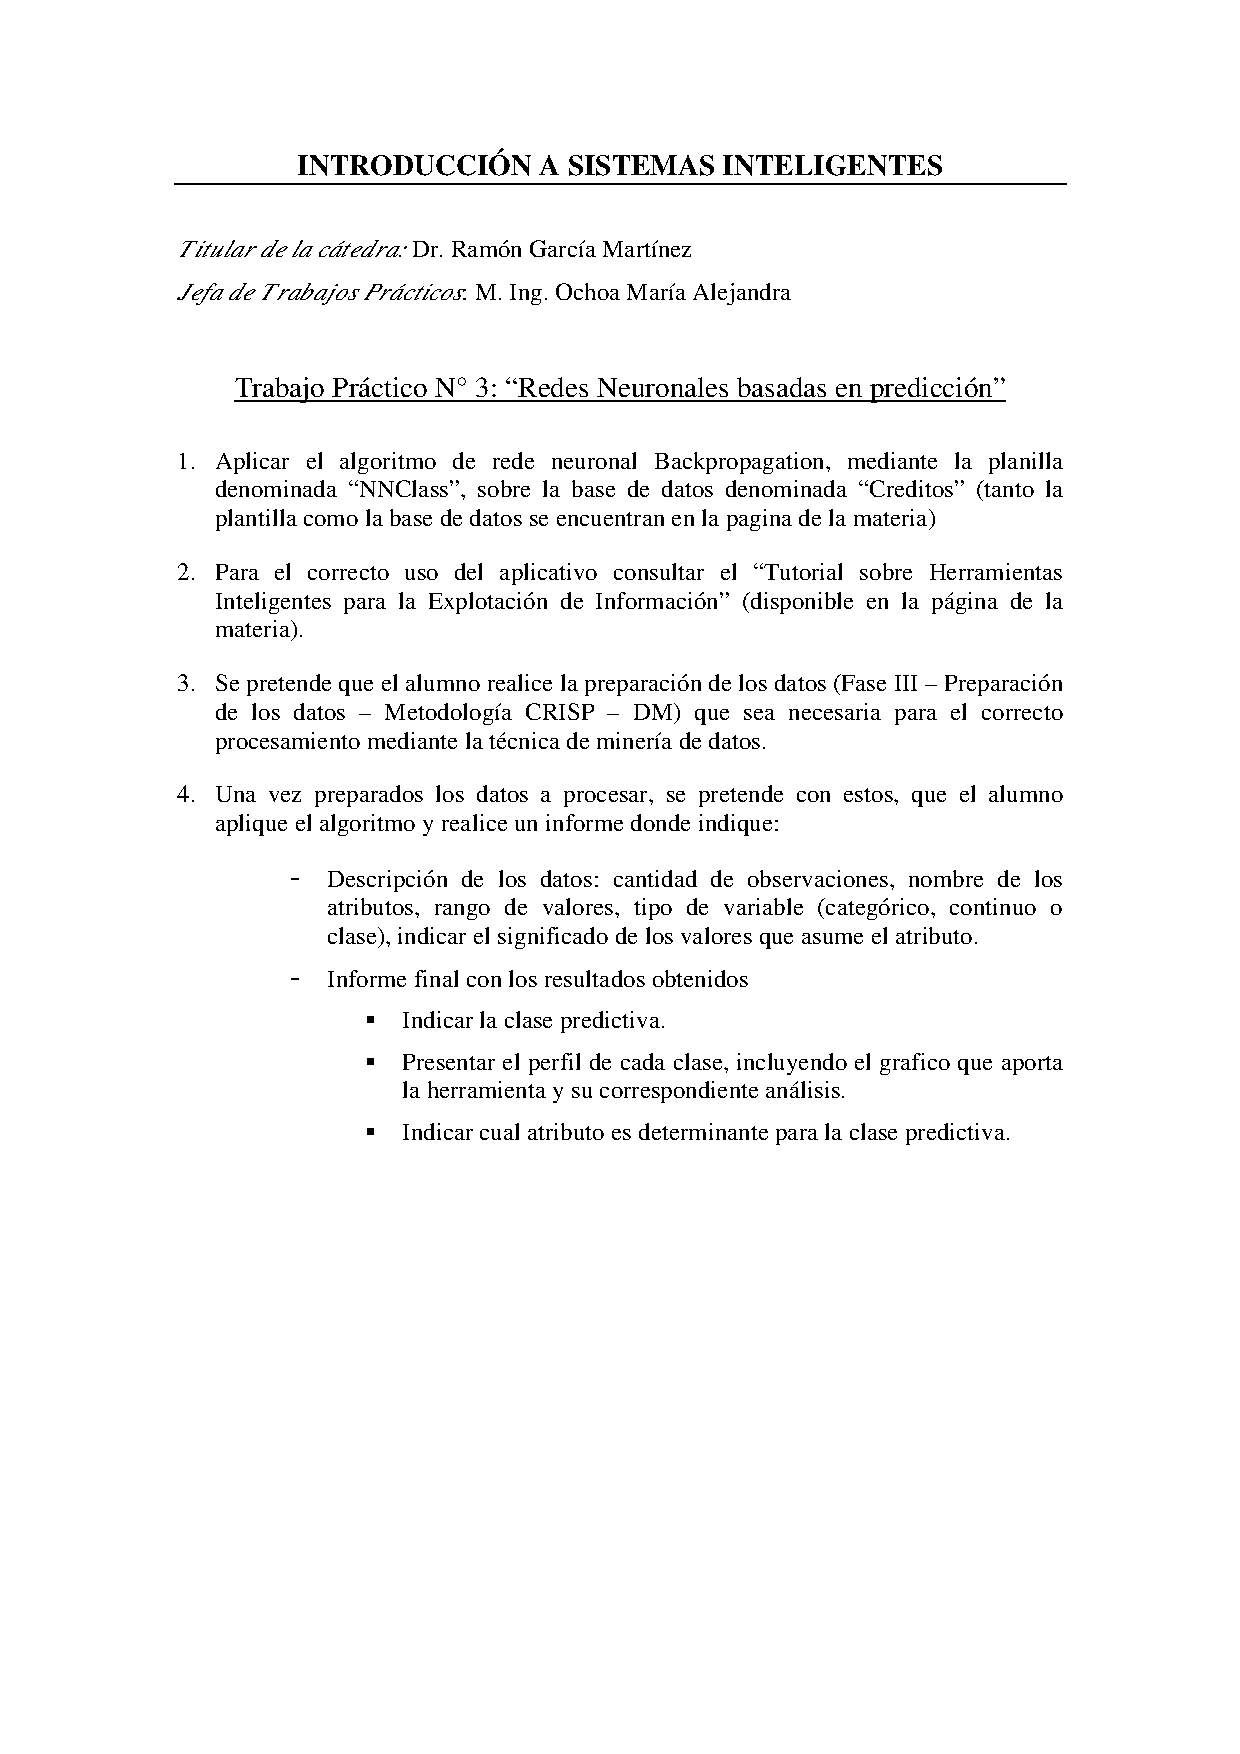
\includepdf[pages={-}, frame=true, pagecommand={}, noautoscale=true, scale=0.7]{doc/enunciado.pdf}

\clearpage

\section{\textbf{Forma de presentación del trabajo práctico}}

\begin{enumerate}
\item Presentar el diagrama de entidad - interrelación con indicaciones de restricciones 
de cardinalidad. 

\item Indicar dependencias de identidad y de existencia en el modelo. 

\item Especificar supuestos que justifiquen el modelo (Hipótesis). 

\item Presentar el diccionario de datos del diagrama con la siguiente información: 

Para cada tipo de entidad se debe especificar:

\begin{enumerate}
\item Definición. 

\item Especificación de atributos. 

\item Especificación de identificador único. 

Para cada tipo de interrelación se debe especificar: ~ 

\item Definición. 

\item Especificación de atributos. 

\item Especificación de identificador único. 
\end{enumerate}

\item Presentar el modelo Relacional ( \texttt{"}de tablas\texttt{"} )~ indicando 
para cada esquema de relación: 

\begin{enumerate}
\item Atributos 

\item Claves candidatas

\item Clave primaria

\item Claves foráneas 

\item Atributos que pueden tomar valores nulos

\item Realice el diagrama del Modelo de Tablas

\item Sentencias DDL
\end{enumerate}
\end{enumerate}

Nota: en los casos en que existan diferentes alternativas para efectuar la transformación 
de MER al modelo de tablas, elegir una única alternativa y enumerar las ventajas 
y desventajas de la alternativa elegida. \pagebreak{}\label{HToc293405800}

\end{document}
